\documentclass[a4paper]{beamer}
%
% Josef Hlavac & Tomas Zahradnicky (21.10.2010)
%
%\usepackage{pgfpages}
%\pgfpagesuselayout{4 on 1}[a4paper,border shrink=5mm,landscape]
%\pgfpagesuselayout{resize}[a4paper,border shrink=5mm,landscape]
\usepackage[utf8]{inputenc}
\usepackage{color}
\usetheme{Frankfurt}
\usecolortheme{whale}
\useinnertheme{circles}
\usepackage{subfigure}
\usepackage[czech,slovak,english]{babel}
%\useinnertheme{rounded}
\usefonttheme{professionalfonts}
\usepackage{bm}
\usepackage{fixltx2e}
\usepackage{minted}
% Multiple rows in the table
\usepackage{multirow}
%
\def\uv#1{\char92\relax #1\char34\relax}
%%%%%%%%%%%%%%%%%%%%%%%%%%%%%%%%%%%%%%%%%%%%%%%%%%%%%%%%%%%%%%%%%%
% Disable the navigation bar in bemaer
\beamertemplatenavigationsymbolsempty
% Useful TODO command
\newcommand{\todo}[1]{\noindent\fbox{\parbox{0.9\textwidth}{\color{red} \bf TODO: #1}\newline}}
% Counter for remarks
\newcounter{RemarkCounter}
%Item which fills the place
\newcommand{\fitem}[0]{\vfill\item}
% Define new column type (align to center in horizontal and vertical position)
\usepackage{array}% http://ctan.org/pkg/array
\newcolumntype{C}{>{\centering\arraybackslash} m{6cm} }
% Helping command for making of more space in the table
\newcommand\T{\rule{0pt}{2.3ex}}
%%%%%%%%%%%%%%%%%%%%%%%%%%%%%%%%%%%%%%%%%%%%%%%%%%%%%%%%%%%%%%%%%%
\newcommand\Title{Ing.}
\newcommand\FirstName{Pavel}
\newcommand\FirstNameAbbreviated{P}
\newcommand\LastName{Benáček}
\newcommand\Email{pavel.benacek@fit.cvut.cz}
\newcommand\DissertationTitle{Generation of High-Speed Network Device from High-Level Description}
%\newcommand\Department{Department of Theoretical Computer Science}
\newcommand\Department{Department of Digital Design}
%\newcommand\Department{Department of Software Engineering}
%\newcommand\Department{Department of Computer Systems}
\newcommand\Faculty{Faculty of Information Technology}
\newcommand\University{Czech Technical University in Prague}
\newcommand\FacultyAndUniversityAbbr{FIT CTU}
%%%%%%%%%%%%%%%%%%%%%%%%%%%%%%%%%%%%%%%%%%%%%%%%%%%%%%%%%%%%%%%%%%
\subject{Generation of High-Speed Network Device from High-Level Description}
\author[\FirstNameAbbreviated. \LastName]{
% My name
Student: \Title{}\,\FirstName{} \LastName{} \\ 
% Supervisor
Supervisor: doc.\,Ing.\,Hana Kubátová,\,CSc. \\ 
% Co-supervisor
Co-Supervisor: Ing.\,Viktor Puš,\,Ph.D.
}

\title{\DissertationTitle}
\titlegraphic{
\includegraphics[width=1.5cm]{logo/LogoCVUT.pdf}}
\institute[\FacultyAndUniversityAbbr]{\Department\\ \Faculty\\ \University}
\date{March 22, 2017}
% Setup the number of frames (current/total)
\setbeamertemplate{footline}[frame number]

% Title page
\begin{document}
\begin{frame}
    \titlepage
\end{frame}

%\section{Outline}
%\subsection*{Outline}
%\begin{frame}
%\frametitle{Outline}
%\tableofcontents
%\end{frame}

% Basic body of presentation
\section{Motivation}
\subsection*{Contributions}
\begin{frame}
    \frametitle{Contributions}
    \begin{itemize}
        \fitem \textbf{Keywords}: FPGA, P4, Mapping to VHDL model, 100\,Gbps
        \fitem \textbf{My research is focused on mapping of abstract description to VHDL model of high-speed network device}
        \fitem I provided the following:
        %
        \begin{enumerate}
            \fitem Modular architecture of high-speed network device (\textbf{100\,Gbps} and beyond)
            \fitem Process of mapping from \textbf{P4 language} (introduced in 2013) to the architecture of high-speed network device
            \fitem Tool --- for verification of architecture and mapping process
            \fitem Overview of usage of High Level Synthesis (C/C++) in high throughput designs. 
            Results of this research were used in other research projects
        \end{enumerate}
    \end{itemize}
    \begin{block}{Contribution to the current state-of-the-art}
        I provided higher degree of flexibility to generation of FPGA based network devices from abstract description (P4 language).
    \end{block}
\end{frame}

\begin{frame}
    \frametitle{Motivation}
    \begin{itemize}
        \fitem Network devices with fixed functionality are not sufficient
        \fitem SDN (Software Defined-Networking)
        \begin{itemize}
            \fitem Promises higher degree of flexibility 
            \fitem Two components --- SDN Controller and SDN Datapath
            \fitem ($\bm{+}$) Application is implemented in controller
            \fitem ($\bm{+}$) Datapath is reconfigurable 
            \fitem ($\bm{-}$) HW devices support a limited set of protocols and actions
        \end{itemize}
        
        \fitem Current requirements on modern network devices
        \begin{itemize}
            \fitem Easy extensibility with new protocols and actions
            \fitem Capability to process data at high rates (100\,Gbps and beyond)
        \end{itemize}
        
        \fitem \textit{Field Programmable Gate Array} (FPGA) provides a reprogrammable structure $\rightarrow$ suitable as a target technology 
        \begin{itemize}
            \fitem Programmed in Hardware Description Language (HDL)
            \fitem Hard to learn
        \end{itemize}
    \end{itemize}
\end{frame}
\section{Background}
\subsection*{Fundamental Network Operations}
\begin{frame} %[allowframebreaks]
    \frametitle{Fundamental Network Operations}
    \begin{itemize}
       \fitem Fundamental network operations from the packet processing point of view
       \begin{enumerate}
           \fitem \textbf{Data Extraction} --- extraction of interesting data (i.e, protocol headers) from incoming packets
           \fitem \textbf{Classification} --- categorization of incoming packets into classes (based on extracted data)
           \fitem \textbf{Data Processing} --- perform an operation based on the assigned class (e.g., data modification, filtering, and so on)
        \end{enumerate}

        \fitem These network operations are the core of each network device
        \fitem Each operation has an influence on throughput        
    \end{itemize}
\end{frame}

\subsection*{Languages and Abstractions}
\begin{frame}[allowframebreaks]
    \frametitle{Languages and Packet Processing Abstractions}
    \begin{itemize}
        \fitem Current HLS tools - not suitable for describing high-speed network devices 
        \begin{itemize}
            \fitem The result highly depends on provided description 
            \fitem Not suitable for novices
        \end{itemize}
        %
        \fitem This drives researchers to provide domain specific languages which are suitable for computer networks 
        \fitem Such languages typically describe packet processing using the match and action model
        \begin{enumerate}
            \fitem \textbf{Gorilla}
            \begin{itemize}
                \fitem Lavasani et al. introduce the language and translation to Verilog
                \fitem Capable to hit 100\,Gbps 
                \fitem Uses templates of processing engines and packet parsers $\rightarrow$ makes the approach somewhat static 
                \fitem e.g., you have to implement the protocol parser if you want to support it
            \end{itemize}
            
            \pagebreak
            
            \fitem \textbf{SDNet}
            \begin{itemize}
                \fitem Commercial solution from Xilinx
                \fitem Introduces the PX language and translation to Verilog
                \fitem Flexible solution capable to scale from 1 to 100\,Gpbs
                \fitem Closed system $\rightarrow$ harder implementation of novel packet processing approaches 
                (not suitable for researchers)
            \end{itemize}
            
            % Put the P4 to the next slide
            \fitem \textbf{P4} (Programming Protocol-independent Packet Processors)
            \begin{itemize}
                \fitem High-level and platform-agnostic language which is developed since 2013
                \fitem Provides a way to define a packet processing functionality
                \fitem Designed to be platform independent (CPU, NPU, ASIC, FPGA)
            \end{itemize}
            
        \end{enumerate}
    \end{itemize}
\end{frame}

\subsection*{Specification of P4 Language}
\begin{frame}
    \frametitle{P4} 
    \framesubtitle{Popularized in  [P4CES16], [ROOT16]}
    \begin{itemize} 
        \fitem Relatively simple syntax\footnote{Specification of the language is available at \url{www.p4.org}}
        \fitem The language defines five basic aspects of packet processing:
        \begin{enumerate}
            \fitem \textbf{Header Format} --- defines the structure of protocol
            \fitem \textbf{Packet Parser} --- defines the process of header parsing
            \fitem \textbf{Table Specification} --- defines how extracted fields are mapped to actions
            \fitem \textbf{Action Specification} --- defines compound actions that may be executed for packets
            \fitem \textbf{Control Program} --- defines the control flow among the tables
        \end{enumerate} 
        \fitem Front end of the compiler is available under open source license 
        $\rightarrow$ compilers for different targets can be implemented      
        \fitem The next step in the SDN ecosystem $\rightarrow$ provides a way for the specification
        of SDN Datapath functionality
    \end{itemize}
\end{frame}

\subsection*{Example}
\begin{frame}[fragile,allowframebreaks]
    \frametitle{Example of P4 Program}
    \framesubtitle{Simple VLAN Tagging Device}
    % Include the file with example
    % Headers and parser % % % % % % % % % % % % % % %
\begin{minipage}[t]{0.48\textwidth}
\begin{minted}[fontsize=\scriptsize]{C}
header_type ethernet_t {
  fields {
    dAddr : 48; 
    sAddr : 48; 
    eType : 16; 
  }   
}

header_type vlan_tag_t {
  fields {
    pcp   : 3;
    cfi   : 1;
    vid   : 12; 
    eType : 16; 
  }   
}
\end{minted}
\end{minipage} 
%
\begin{minipage}[t]{0.48\textwidth}
\begin{minted}[fontsize=\scriptsize]{C}
parser start {
  return parse_ethernet;
}

header ethernet_t eth;
parser parse_ethernet {
  extract(eth);
  return select(latest.eType) {
    0x8100  : parse_vlan;
    default : ingress;
  }   
}

header vlan_tag_t vlan;
parser parse_vlan {
  extract(vlan);
  return ingress;
}   
\end{minted}
\end{minipage}

\pagebreak

% Actions, control, Table % % % % % % % % % % % % % % %
\begin{minipage}[t]{0.48\textwidth}
\begin{minted}[fontsize=\scriptsize]{C}
control ingress {
  if(valid(vlan)) {
    // We want to retag or
    // add a tag based on
    // the source MAC
    apply(retagTable);
  } else {
    // We want to add
    // the tag
    apply(tagTable);
  }
}

table retagTable {
  reads {
    vlan.vid : exact;
  }
  actions {retag; remove;}
}
\end{minted}
\end{minipage}
\begin{minipage}[t]{0.48\textwidth}
\begin{minted}[fontsize=\scriptsize]{C}
table tagTable {
  reads {
    eth.sAddr : exact;
  }
  actions {add;}
}
 
function retag(vid) {
  modify_field(vlan.vid,vid);
}

function remove() {
  modify_field(eth.eType,vlan.eType);
  remove_header(vlan);
}

function add(vid) {
  add_header(vlan);
  ...
}
    \end{minted}
\end{minipage} 
\end{frame}
\section{Main Content}
\subsection*{Top Level Architecture of Network Device}
\begin{frame}
    \frametitle{Basic Overview}
    \framesubtitle{Published in [MICPRO16] journal}
    %
    \begin{itemize}
        \fitem Current HLS tools are sensitive to provided input
        \fitem Controlled mapping process
        \begin{itemize}
            \fitem We can control the architecture generation process
            \fitem Easier to sustain parameters of generated network device (frequency, consumed resources)
        \end{itemize}
       
        \fitem The most modern abstract language is used (P4; since 2013)
        \fitem The mapping requires:
        \begin{enumerate}
            \fitem Modular target architecture of high-speed network device
            \fitem Identification of building macro blocks which are combination of optimized hand-written and generated code
        \end{enumerate}
        
        \fitem This approach allows:
        \begin{enumerate}
            \fitem Minimization of suboptimal input from the user
            \fitem Keep the quality of generated code (compared to hand-written)
            \fitem Rapid prototyping of high-speed network devices
            \begin{itemize}
                \fitem Many lines of HDL code are generated in short time
            \end{itemize}
        \end{enumerate}
    \end{itemize}
\end{frame}

\begin{frame}
    \frametitle{Use Case Study}
    \framesubtitle{Generated Code vs. Total Lines of Code}
    
    \begin{enumerate}
        \fitem \textbf{IPv4 Filter} --- filtering of packets is based on the IPv4 address, the non-IP traffic is dropped
        \fitem \textbf{IPv4+IPv6 Filter}  --- extends the IPv4 Filter with further support of IPv6 protocol, the non-IP traffic is dropped
        \fitem \textbf{Full Filter} --- extends the IPv4+IPv6 Filter with further support of tagging (VLAN and MPLS)
    \end{enumerate}
    
    
    \begin{table}
        \footnotesize
        \centering
        \begin{tabular}{|l||c|c||c|c|}
            \hline
            \T \textbf{Project} & \textbf{P4 lines} & \textbf{Time\,[s]} & \textbf{Generated lines} & \textbf{Total lines} \\ \hline\hline
            \T IPv4 Filter      &        91         &       1.574        &           6283           &        24791         \\
            IPv4+IPv6 Filter    &        129        &       1.818        &           9888           &        28396         \\
            Full Filter         &        212        &       1.929        &          13824           &        32332         \\ \hline
        \end{tabular}
    \end{table}
    
    \begin{itemize}
        \footnotesize
        \fitem \textbf{P4 lines} --- the number of lines of P4 source code
        \fitem \textbf{Time} --- the time required for the translation
        \fitem \textbf{Generated lines} --- expresses the effort of the generator
        \fitem \textbf{Total Lines} ---  the sum of generated lines and lines of library source code (FIFO, TCAM, and so on)
    \end{itemize}
\end{frame}

\begin{frame} %[allowframebreaks]
    \frametitle{Target Architecture}
    \framesubtitle{Published in [H2RC16]}
    {
    \hspace*{-26pt}
    
\includegraphics[width=1.15\textwidth]{pic/p4-pipeline}
    }
\end{frame}

\subsection*{Parser}
\begin{frame}
    \frametitle{Parser}
    \framesubtitle{Published in [FCCM16], [H2RC15], [H2RC16], [MICPRO16] journal, [P4ST16]}
    \begin{itemize}
        \fitem The architecture is inspired by the work of Puš et al.
        \begin{itemize}
            \scriptsize
            \fitem[$\rightarrow$]  Viktor Puš, Lukáš Kekely and Jan Kořenek. \textit{Design methodology of configurable high performance packet parser for FPGA}. 17th International Symposium on Design and Diagnostics of Electronic Circuits \& Systems, 2014.
        \end{itemize}
        \fitem Authors do not present the mapping from abstract description
        \begin{itemize}
            \fitem I identified fundamental block types (generated, configured and static)
            \fitem I provided an elegant mapping of P4 source code to fundamental blocks
        \end{itemize}
        
        \fitem The generated parser is a combination of:
        \begin{itemize}
            \fitem Hand-written code (optimized) --- used for static and configured blocks
            \fitem Generated code --- protocol specific code
        \end{itemize}        
        %\fitem Generated parsers (FPGA) are approximately two times bigger and have higher latency
        \fitem Generated parsers are bigger and have higher latency $\rightarrow$ cost for flexibility
    \end{itemize}
\end{frame}

\begin{frame}
    \frametitle{Parser --- Consumed Resources}
    \framesubtitle{Hand-written vs. Generated Parsers (the same protocol set)}
    
    \begin{figure}[t]
        \centering
        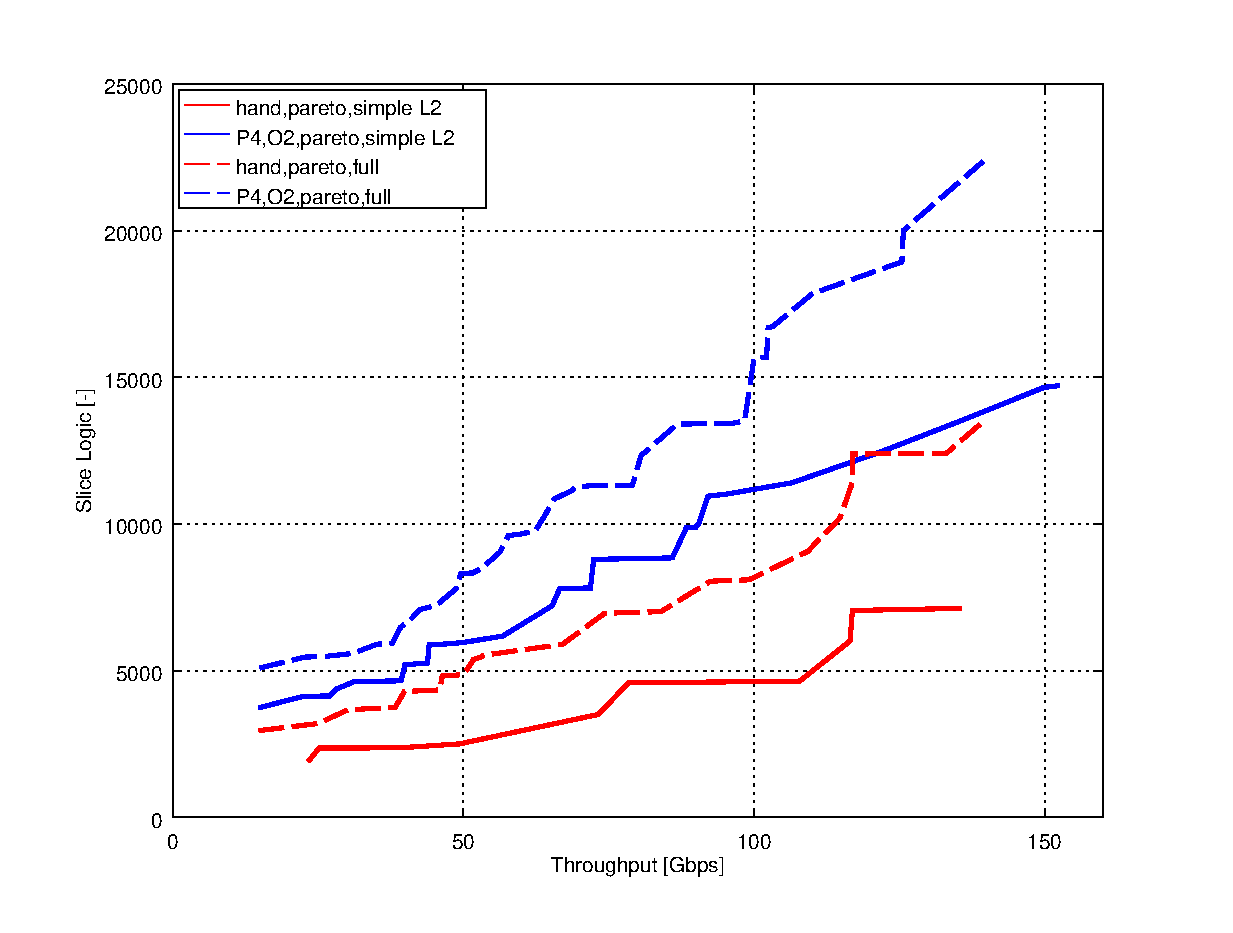
\includegraphics[width=0.89\textwidth]{pic/graph/hfe/1_thrslice_logic_pareto}
    \end{figure}
\end{frame}

\begin{frame}
    \frametitle{Parser --- Latency}
    \framesubtitle{Hand-written vs. Generated Parsers (the same protocol set)}
    
    \begin{figure}[t]
        \centering
        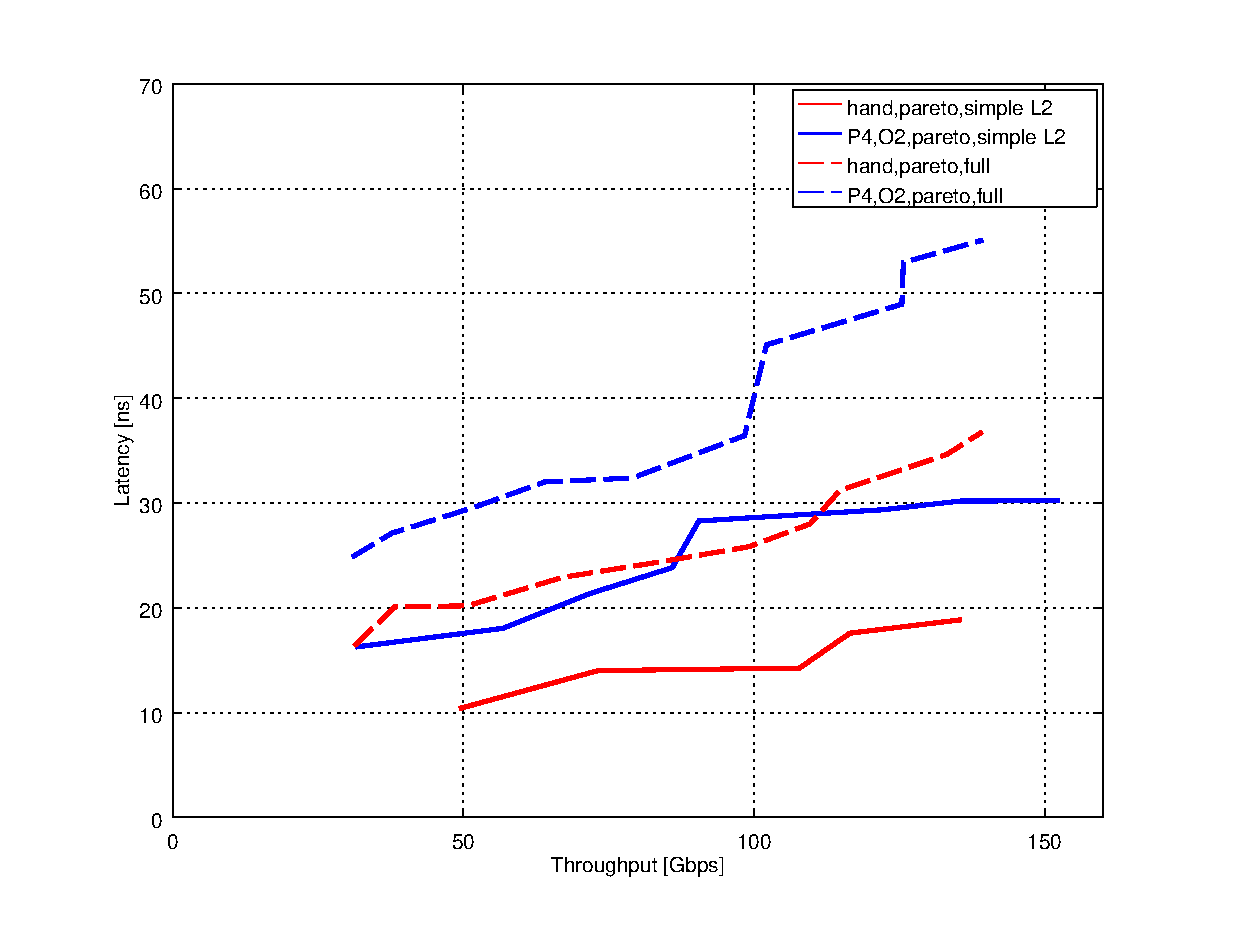
\includegraphics[width=0.89\textwidth]{pic/graph/hfe/2_thrlat_pareto}
    \end{figure}
\end{frame}

\subsection*{Deparser}
\begin{frame}
    \frametitle{Deparser}
    \framesubtitle{Published in [H2RC16], [P4ST16], [MICPRO16] journal}
    \begin{itemize}
        \fitem Deparsing $\rightarrow$ the reverse operation to parsing
        %\fitem In my best knowledge, I provided the first architecture and experimental results 
        \fitem I provided the following:
        \begin{itemize}
            \fitem Architecture of fundamental building blocks (configured and generated)
            \fitem The process of mapping from P4 to fundamental building blocks
        \end{itemize}
        
        \fitem The deparsing process is optimized to minimize consumed resources
        \begin{itemize}
            \fitem Protocol header is inserted \textbf{before} the payload
            \fitem Protocol with \textbf{fixed} length (e.g., Ethernet) --- shifting logic is simple
            \fitem Protocol with \textbf{variable} length (e.g., IPv4) --- shifting logic has to support several offsets for payload
        \end{itemize}
        
        \fitem The current architecture of deparser is inefficient when deparsing short frames 
    \end{itemize}
\end{frame}

\begin{frame}
    \frametitle{Deparser --- Consumed Resrouces}
    \framesubtitle{Generated Deparsers}
    
    \begin{figure}[t]
        \centering
        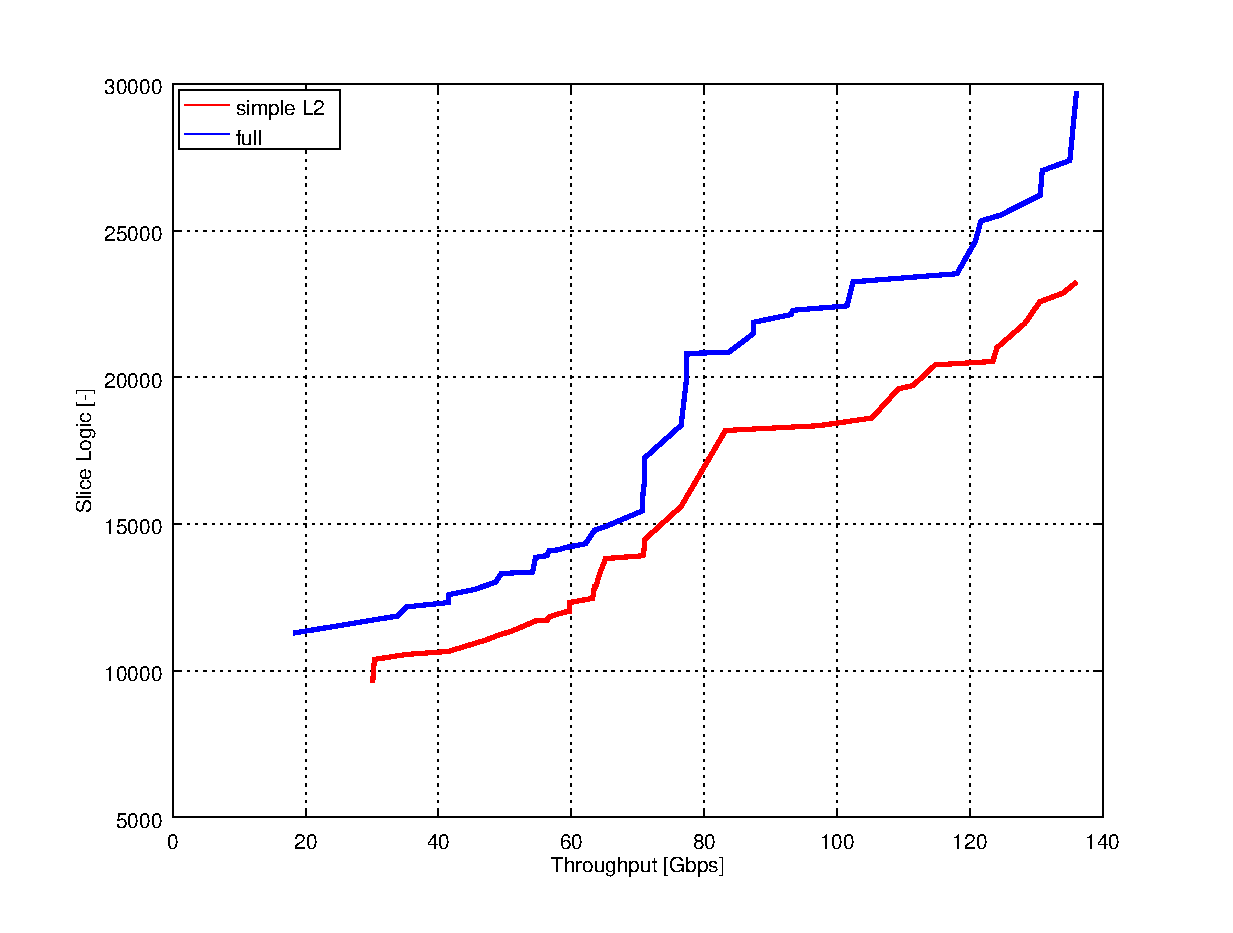
\includegraphics[width=0.89\textwidth]{pic/graph/deparser/1_thr_slice_logic_pareto}
    \end{figure}
\end{frame}

%\begin{frame}
%    \frametitle{Deparser --- Latency}
%    \framesubtitle{Generated Deparsers}
%    
%    \begin{figure}[t]
%        \centering
%        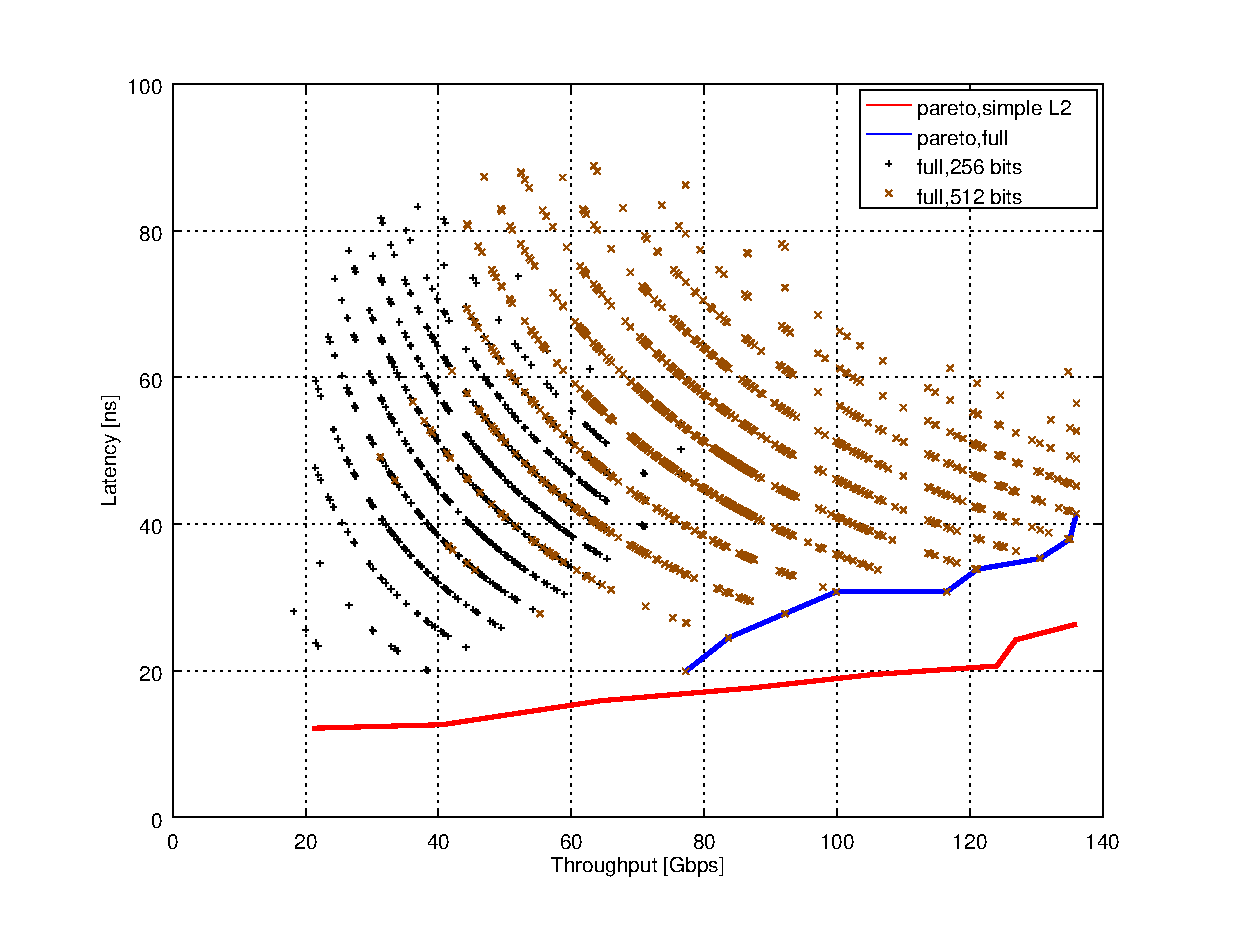
\includegraphics[width=0.89\textwidth]{pic/graph/deparser/3_thr_latency_deparser}
%    \end{figure}
%\end{frame}

\subsection*{Match+Action}
\begin{frame}
    \frametitle{Match+Action}
    \framesubtitle{Published in [MICPRO16], [H2RC16], [FPL13], [ANCS14], [MEMICS14], [FPGA14]}
    
    %\todo{Sem dat info o match+action, prvni implementace, mapovane komplet z vhdl, propustnost 100gbps, ukazano na trech use casech}
    \begin{itemize}
        \fitem Implements the \textbf{Match} (i.e., searching for the most suitable rule) and \textbf{Action} (i.e., data modification) functionality
        \begin{itemize}
            \fitem Search algorithms are out of scope of my work
        \end{itemize}
        %
        \fitem Modular architecture of Match+Action pipeline, designed to process 100\,Gbps and beyond
        \fitem I provided the following:
        \begin{itemize}
            \fitem Architecture of fundamental building blocks (configured, generated and mixed)
            \fitem The process of mapping from P4 to fundamental building blocks
        \end{itemize}
        %
        \fitem Optional usage of HLS for easy extensibility of action set
        \begin{itemize}
            \fitem Based on my research for DMON100 project\footnote{More information available from \url{http://dmon100.liberouter.org/}}
            \fitem I use C/C++ for description of complex processing at speed of 100\,Gbps
            \fitem Allows us extend the action set of P4 language in shorter time
        \end{itemize}
        %
        %\fitem Experiments --- to address consumed resources and throughput of generated P4 pipelines
    \end{itemize}
\end{frame}

\begin{frame}
    \frametitle{Generated P4 Pipelines --- Consumed Resources}
    \framesubtitle{Published in [MICPRO16] journal,[H2RC16]}
    
    \begin{figure}
        \centering
        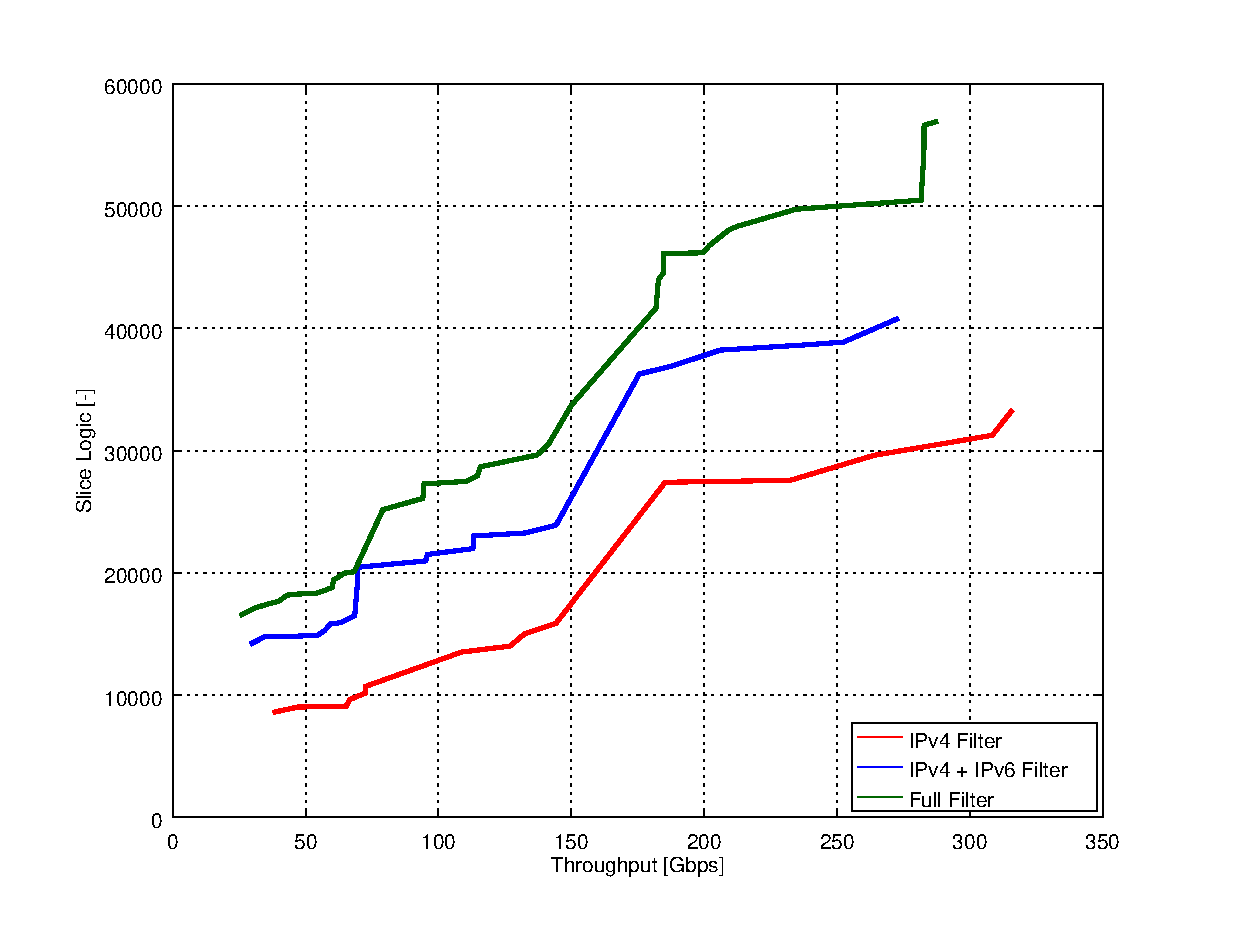
\includegraphics[width=0.89\textwidth]{pic/graph/table/thr_slice_logic_pareto}
    \end{figure}
\end{frame}

\begin{frame}[allowframebreaks]
    \frametitle{Generated P4 Pipelines --- Throughput}
    \framesubtitle{Published in [MICPRO16] journal}
    
    \begin{figure}
        \centering
        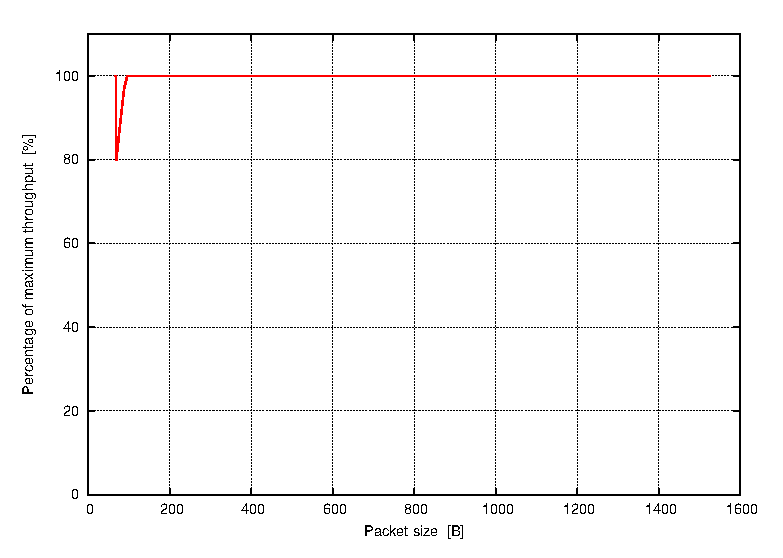
\includegraphics[width=0.89\textwidth]{pic/graph/table/ipv46_throughput}
    \end{figure}
    
    \begin{figure}
        \centering
        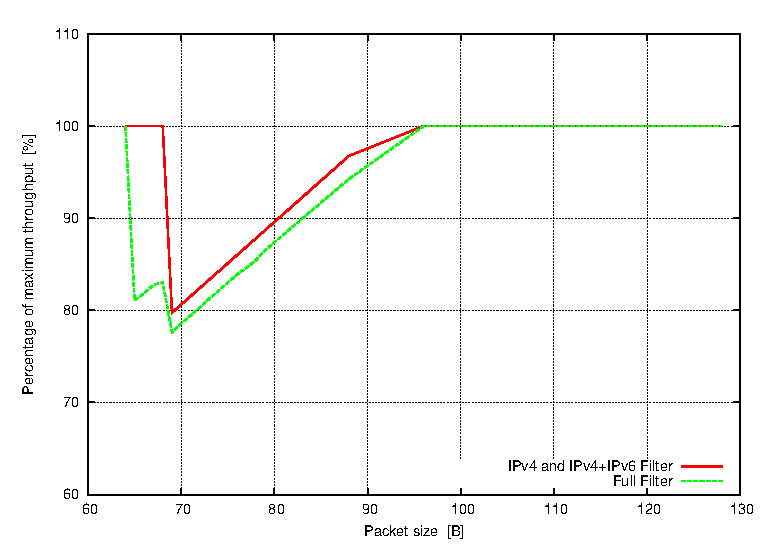
\includegraphics[width=0.89\textwidth]{pic/graph/table/detail_throughput_ineff}
    \end{figure}
\end{frame}

\subsection*{Comparison with Related Work}
\begin{frame}
    \frametitle{Comparison with Related Work}
    \framesubtitle{P4 $\rightarrow$ Bluespec}
    \begin{itemize}
        \fitem The nearest comparable solution: mapping P4 $\rightarrow$ Bluespec\footnote{More information available from \url{http://www.bluespec.com/}}
        \begin{itemize}
            \footnotesize
            \fitem[$\rightarrow$] Wang, Han, et al. \textit{P4FPGA: A Rapid Prototyping Framework for P4}. ACM SOSR 2017 Symposium on SDN research, Santa Clara, CA, USA, 2017.
        \end{itemize}
        %
        \fitem Their solution:
        \begin{itemize}
            \fitem Supports both versions of P4 language (P4\textsubscript{14} and P4\textsubscript{16})
            \fitem Supports API for easy configuration of network device
            \fitem Supports simple stateful processing
            \fitem No demonstration of advanced deparsing
        \end{itemize}
        \fitem My solution:
        \begin{itemize}
            \fitem Higher throughput (60\,Gbps vs. 100\,Gbps and beyond)
            \fitem No additional tool is needed (Bluespec $\rightarrow$ Verilog)
            \fitem Capable to reach higher frequencies on slower FPGA
            \fitem Throughput of parser is protocol independent
        \end{itemize}
            
    \end{itemize}
\end{frame}

\section{Conclusion and Contributions}
\subsection*{Conclusion and Contributions}
\begin{frame}
    \frametitle{Conclusion and Contributions}
    \begin{itemize}
        \fitem \textbf{My research is focused on mapping of abstract description to VHDL model of high-speed network device}
        \fitem I provided the following:
        %
        \begin{enumerate}
            \fitem Modular architecture of high-speed network device (\textbf{100\,Gbps} and beyond)
            \fitem Process of mapping from \textbf{P4 language} (introduced in 2013) to the architecture of high-speed network device
            \fitem Tool --- for verification of architecture and mapping process
            \fitem Overview of usage of High Level Synthesis (C/C++) in high throughput designs. 
            Results of this research were used in other research projects. 
        \end{enumerate}
        %
        \fitem The quality of generated code is comparable to hand-written one
        \begin{itemize}
            \fitem More resources are the cost for flexibility
        \end{itemize}
        \fitem The result of this research was verified against real network test devices
    \end{itemize}
\end{frame}

\subsection*{Publications and Evaluation Activities}
\begin{frame}[allowframebreaks]
    \frametitle{Publications and Evaluation Activities}
    %
    {
    % Use the small font in all publications
    \footnotesize
    \textbf{\underline{Reviewed Publications of the Author Relevant to the Thesis}}
    \begin{itemize}
        \fitem[$\rightarrow$] \textbf{[FCCM16]} P. Ben\'{a}\v{c}ek, V. Pu\v{s} and H. Kub\'{a}tov\'{a}.
        \textit{P4-to-VHDL: Automatic Generation of 100Gbps Packet Parsers}. IEEE 24\textsuperscript{th} Annual International Symposium on Field-Programmable Custom Computing Machines (FCCM2016), Washington D.C., USA, 2016.
        %
        \fitem[$\rightarrow$] \textbf{[H2RC15]} P. Ben\'{a}\v{c}ek, V. Pu\v{s} and H. Kub\'{a}tov\'{a}. \textit{Automatic Generation of 100 Gbps Packet Parsers from P4 Description}.
        First International Workshop on Heterogeneous High-performance Reconfigurable Computing, Austin, TX, USA, 2015.
        %
        \fitem[$\rightarrow$] \textbf{[DSD14]} P. Ben\'{a}\v{c}ek, H. Kub\'{a}tov\'{a} and V. Pu\v{s}. \textit{Architecture of Effective High-Speed Network Stream Merger}.
        Digital System Design (DSD), 17\textsuperscript{th} Euromicro Conference on Digital System Design, pp. 459--464, Verona, Italy, 2014.
        %
        \fitem[$\rightarrow$] \textbf{[FPGA14]} P. Ben{\'a}{\v{c}}ek and V. Pu{\v{s}}.
        \textit{Application specific processor with high-level synthesized instructions}.
        ACM/SIGDA international symposium on Field-Programmable Gate Arrays, pp. 246--246, Monterey, CA, USA,
        2014.
        %
        \fitem[$\rightarrow$] \textbf{[ANCS14]} P. Ben\'{a}\v{c}ek, T. \v{C}ejka, H. Kub\'{a}tov\'{a} and R. Bla\v{z}ek.
        \textit{Change-Point Detection Method on 100 Gb/s Ethernet Interface}.
        ACM/IEEE Symposium on Architectures for Networking and Communications Systems, Marina del Rey, CA, USA,
        2014.
        \smallskip \\ The paper has been cited in:
        \begin{itemize}
            \footnotesize
            \fitem Nakamura, Kohei, Ami Hayashi, and Hiroki Matsutani. \textit{An FPGA-Based Low-Latency Network Processing for Spark Streaming}. Proceedings of the Workshop on Real-Time and Stream Analytics in Big Data (IEEE BigData 2016 Workshop), 2016.
        \end{itemize}
        %
        \fitem[$\rightarrow$] \textbf{[MEMICS14]} P. Ben\'{a}\v{c}ek, T. \v{C}ejka, H. Kub\'{a}tov\'{a}, L. Kekely and R. Bla\v{z}ek.
        \textit{FPGA Accelerated Change-Point Detection Method for 100 Gb/s Networks}.
        Doctoral Workshop on Mathematical and Engineering Methods in Computer Science, Tel\v{c}, Czech Republic,
        2014.
        %
        \fitem[$\rightarrow$] \textbf{[H2RC16]} P. Ben\'{a}\v{c}ek, V. Pu\v{s} and P. Ka\v{s}tovsk\'y.
        \textit{P4-to-FPGA: High Performance Reconfigurable Networking (poster)}.
        Second International Workshop on Heterogeneous High-performance Reconfigurable Computing, Salt Lake City, UT, USA,
        2016.
        %        
        \fitem[$\rightarrow$] \textbf{[P4ST16]} P. Ben{\'a}{\v{c}}ek and V. Pu{\v{s}}.
        \textit{P4-to-VHDL: Generating High Speed Network Devices (poster)}. 
        P4 Workshop, Stanford, California, USA, 
        2016.
        %
        \fitem[$\rightarrow$] \textbf{[FPL13]} L. Kekely, V. Pu\v{s}, P. Ben{\'a}\v{c}ek and J. Ko\v{r}enek.
        textit{Trade-offs and progressive adoption of FPGA acceleration in network traffic monitoring}.
        Field Programmable Logic and Applications (FPL), 24\textsuperscript{th} International Conference, pp. 1--4, Munich, Germany,
        2014.
        \smallskip \\ \smallskip The paper has been cited in:
        \begin{itemize}
            \footnotesize
            \item D. Grochol, L. Sekanina, M. \v{Z}\'{a}dn\'{i}k, J. Ko\v{r}enek. \textit{Evolutionary circuit design for fast FPGA-based classification of network application protocols}. 
            Applied Soft Computing, Volume 38, January 2016, pp. 933-941.
            \item L. Tang, J. Yan, Z. Sun, T. Li, M. Zhang. \textit{Towards high-performance packet processing on commodity multi-cores: current issues and future directions}.
            Research Paper Special Focus On Future Internet Architecture And Protocol Science China Information Sciences, December 2015, Volume 58, Issue 12, pp. 1-16.
        \end{itemize}
    \end{itemize}
    %
    \textbf{\underline{Submitted Publications}}
    \begin{itemize}
        \fitem[$\rightarrow$] \textbf{[MICPRO16]} P. Ben\'{a}\v{c}ek, H. Kub\'{a}tov\'{a} and V. Pu\v{s}.
        \textit{P4-to-VHDL: Automatic Generation of High-Speed Input and Output Network Blocks}.
        Microprocessors and Microsystems, Elsevier Journal, 2016.
    \end{itemize}
    %
    \textbf{\underline{Evaluation Activities}}
    \begin{itemize}
      \fitem[$\rightarrow$] Review of article for the \textit{Journal of Parallel and Distributed Computing}. Article in journal, ISSN 0743-7315, 2016.
      %
      \fitem[$\rightarrow$] Conference Programme Committee member in the \textit{Track on Reconfigurable Computing for Networks and Communications}. International Conference on Reconfigurable Computing and FPGAs (ReConFig'2016), Cancun, Mexico, 2016.
    \end{itemize}
    %
    \textbf{\underline{P4 Popularization}}
    \begin{itemize}
        \fitem[$\rightarrow$] \textbf{[ROOT16]} P. Ben{\'a}{\v{c}}ek and V. Pu{\v{s}} 
        \textit{The P4 Language as the Future of SDN (CZ)}. 
        root.cz (part 1 and part 2), 2016.
        %
        \fitem[$\rightarrow$] \textbf{[P4CES16]} P. Ben{\'a}{\v{c}}ek and V. Pu{\v{s}} 
        \textit{The P4 Language as the Future of SDN (CZ)}. 
        CESNET blog, 2016 
       
     \end{itemize}
    } 
\end{frame}



% % % % % % % % % % % % % % % % % % % % % % % % % % % % %  % % DISCUSSION % % % % % % % % % % % % % % % % % % % % % % % % % % % % %
\appendix
%\section{prof.\,Giuseppe Bianchi}
\section{prof.\,Giuseppe Bianchi}
\setcounter{RemarkCounter}{1}
% Prof. Bianchy
\subsection{Remark \theRemarkCounter}
\begin{frame}[allowframebreaks]
    \begin{block}{Remark \theRemarkCounter}
        Did you think about the possibility to include ALUs (Arithmetic and Logic Units) in the
        pipeline in order to further improve programmability? This is (probably, given the very
        obscure and unreliable info available) what the Barefoot PISA chip does (claims to do), and
        would be interesting to compare your architecture with what we can guess the 
        "commercial competitors" do.
    \end{block}
    \begin{exampleblock}{Answer}
        No. All arithmetic and logic operations are known in the time of translation. So,
        there is no need to include complex ALU because all operations are programmed and described in HDL. 
        This approach allows optimization of consumed resources $\rightarrow$ not used operations are not synthesized.
        This is also the advantage of FPGA against ASIC.
    \end{exampleblock}
    
    %\pagebreak
\end{frame}
\stepcounter{RemarkCounter}

\subsection{Remark \theRemarkCounter}
\begin{frame}[allowframebreaks]
    \begin{block}{Remark \theRemarkCounter}
        Somewhat related to the above: P4 includes some instructions which permit some further
        flexibility and programmability also of actions (that's arguably related with the need to
        include ALUs discussed above). Can your approach support "all" the P4
        specifications/instructions or only a subset? If this is the case, can you comment on
        limitations and differences?
    \end{block}
    
    \begin{exampleblock}{Answer}
        The architecture supports a subset of instructions. Packet loopback and packet clone functionality of P4 model are not implemented.
        However, such instructions are mainly the task of infrastructure (around) a P4 pipeline.
        The functionality can be implemented but it can degrade the throughput.
    \end{exampleblock}   
\end{frame}
\stepcounter{RemarkCounter}

\subsection{Remark \theRemarkCounter}
\begin{frame}[allowframebreaks]
    \begin{block}{Remark \theRemarkCounter}
       The SDM approach is not a contribution of this thesis, but is an integral part of your
       approach. Can you please comment on whether you need to adapt the SDM approach, or
       whether you could rely on it with minimal/trivial adaptations? (not fully clear from reading
       the thesis whether you just "used" the SDM approach or needed to further extend it).
    \end{block}
    
    \begin{exampleblock}{Answer}
        %Generally, the SDM approach was known before the P4 and the idea comes from my co-supervisor. 
        My work on HLS allows to extend the SDM with more complex instructions in shorter time.
        This approach can be also used to go beyond a limited set of P4 instructions.
        So, I took results from the previous research and I applied them in my own research.       
%         Generally, the SDM approach was known before the P4 and the idea comes from my co-supervisor. 
%         My work in P4 is based on observations and architectural decisions from the previous research for SDM.
%         So, I adopt the main ideas of general packet processing but I added the flexibility because P4 instructions 
%         are more complex. Moreover, we can use the HLS and go beyond the P4.      
    \end{exampleblock}
\end{frame}
\stepcounter{RemarkCounter}

\subsection{Remark \theRemarkCounter}
\begin{frame}[allowframebreaks]
    \begin{block}{Remark \theRemarkCounter}
         Which challenges and further technical enhancements
         are needed to support stateful processing a la OpenState? It would require a brand new
         design or you believe your architecture can be adapted?        
    \end{block}
    
    \begin{exampleblock}{Answer}
        Current architecture doesn't support the stateful processing a la OpenState. 
        However, I think that the architecture could be extended with OpenState-like processing in Match+Action table 
        $\rightarrow$ we can define the new type of Match+Action table which supports the stateful processing.
    \end{exampleblock}
    
    \pagebreak
    
    \begin{figure}
        \includegraphics[width=\textwidth]{pic/OpenStateConcept}
        \caption{OpenState concept (taken from \url{http://openstate-sdn.org/})}
    \end{figure}
\end{frame}
\stepcounter{RemarkCounter}

%\section{Ing.\,Katar\'{i}na Jelemensk\'{a},\,PhD.}
\section{Ing.\,Katarína Jelemenská,\,PhD.}
\setcounter{RemarkCounter}{1}
% dr. Jelemenska
\subsection{Remark \theRemarkCounter}
\begin{frame}[allowframebreaks]
    \begin{block}{Remark \theRemarkCounter}
        The experiments, discussed in the thesis, are focused mainly on the transformation efficiency
        and the throughput of generated network devices. However, the first thing to prove is the 
        functional correctness. Could you explain, how was the correctness of the transformation 
        process and the generated network devices verified?
    \end{block}
    
    \pagebreak
    
    \begin{exampleblock}{Answer}
        \begin{itemize}
            \fitem \textbf{Block level testing}
                \begin{enumerate}
                    \fitem Functional verification of fundamental idea (for each block) --- manual implementation of first block version + verification environment (similar to \textbf{OVM} - Open Verification Methodology).
                    \fitem Generated block is connected instead of the manual implementation.
                \end{enumerate}
            \fitem \textbf{Integration testing}
                \begin{enumerate}
                    \fitem Manual implementation of functional verification environment for complex (generated) pipelines.
                    \fitem Verification of different use-cases in real environment against the Spirent Test device.
                \end{enumerate}
        \end{itemize}
        
        However, I know that this is not sufficient and it drives me to design the automatic test environment.
    \end{exampleblock}
    
    \pagebreak
    \begin{figure}
        \vspace*{0pt}
        \centering
        
\includegraphics[width=0.99\textwidth]{pic/p4-testbed}
    \end{figure}
      
\end{frame}
\stepcounter{RemarkCounter}

\subsection{Remark \theRemarkCounter}
\begin{frame} %[allowframebreaks]
    \begin{block}{Remark \theRemarkCounter}
        In section 4.1.3 a possibility of P4 program optimization is discussed. It is clear that P4
        program has to be designed manually. However, based on the provided optimization example it
        looks like it could be then optimized automatically. Why is it not possible?
    \end{block}
    
    \begin{exampleblock}{Answer}
        The automation of such optimization is not the part of my thesis because we found the only one specific example (TCP/UDP). 
%        The automation of such optimization wasn't part of my thesis because we identified one 
%        specific example (TCP/UDP).
    \end{exampleblock}

\end{frame}
\stepcounter{RemarkCounter}

\subsection{Remark \theRemarkCounter}
\begin{frame}[allowframebreaks]
    \begin{block}{Remark \theRemarkCounter}
            In most of the related authors publications one of the co-author is Viktor Puš.
            For example the papers A.1 and A.2 resemble the summary of this thesis. 
            Could you strictly distinguish the contribution of the two authors?
    \end{block}
    
    \begin{exampleblock}{Answer}
        Dr.\,Puš came with the main idea of modular parser and he also provided the first manual implementation. The rest of presented work (in the thesis) is mine.
    \end{exampleblock}  
     %\pagebreak
\end{frame}
\stepcounter{RemarkCounter}

%\section{Dr.\,Alistair McEwan}
\section{Dr.\,Alistair McEwan}
\setcounter{RemarkCounter}{1}
%dr. McEwan
\subsection{Remark \theRemarkCounter}
\begin{frame}[allowframebreaks]
    \begin{block}{Remark \theRemarkCounter}
        Chapter 2 discussed the benefits and drawbacks of a variety of languages used in this study,
        and others. However the evaluation of these languages seems rather subjective---based either
        on the authors view, or on the view of those whose work he cites. An example of this is
        Handel-C: the language was intended to make reconfigurable hardware accessible to software
        engineers, rather than focus on performance (and the reviewer published some work in this
        area, specifically relating to the efficiency of CAM architectures on FPGA-based network
        architectures). How might an evaluation of languages in this area be made more objective?
    \end{block}
    
    \pagebreak
    
    \begin{exampleblock}{Answer}
        Reviewer is right that evaluation of discussed languages are based on my and others views. 
        We can do the following for more objective evaluation:
        \begin{enumerate}
            \fitem Obtain a set of problems, languages and developers.
            \fitem Let each developer implements the set of problems in given languages.
            \fitem Finally, we compare parameters of synthesized designs like frequency, consumed resources and time required for development.
        \end{enumerate}
    \end{exampleblock}
\end{frame}
\stepcounter{RemarkCounter}

\subsection{Remark \theRemarkCounter}
\begin{frame}[allowframebreaks]
    \begin{block}{Remark \theRemarkCounter}
        A corollary of the above question concerns the use of T-CAMs in chapter 5. What are the
        trade-offs between a single cycle lookup, hardware costs, latency, and overall throughput?
        It would seem intuitive that a significant amount of actions implemented in a T-CAM could
        considerably skew some of these results.
    \end{block}
    
    \pagebreak
    
    \begin{table}
        \centering
        \footnotesize
        \begin{tabular}{|c|c||c|c|c|}
        	\hline
        	\T\textbf{Search time\,[\# clk.]} & \textbf{\# Entries} & \textbf{LUT} & \textbf{Regs.} & \textbf{Freq.\,[MHz]} \\ \hline\hline
        	      \T\multirow{4}{*}{1}        &         64          &     2015     &      343       &        399.52         \\
        	                                  &         128         &     3807     &      409       &        294.55         \\
        	                                  &         256         &     7395     &      537       &        293.08         \\
        	                                  &         512         &    14587     &      795       &        291.63         \\ \hline
        	                %                 &        1024         &    29143     &      1311      &        291.61         \\
        	                %                 &        2048         &    58049     &      2338      &        291.63         \\
        	      \T\multirow{4}{*}{2}        &         64          &     1384     &      345       &        363.63         \\
        	                                  &         128         &     2551     &      410       &        361.40         \\
        	                                  &         256         &     4608     &      539       &        360.62         \\
        	                                  &         512         &     8939     &      796       &        358.42         \\ \hline
        	                %                 &        1024         &    17667     &      1309      &        356.25         \\
        	                %                 &        2048         &    35339     &      2334      &        366.03         \\
        	      \T\multirow{4}{*}{4}        &         64          &     943      &      346       &        365.23         \\
        	                                  &         128         &     1639     &      411       &        362.97         \\
        	                                  &         256         &     3035     &      540       &        360.75         \\
        	                                  &         512         &     5546     &      797       &        359.97         \\ \hline
        \end{tabular}
        \caption{Required resources of used TCAM (132 bit search key)}
     \end{table}
     % Insert the enumeration to minipage because we want to move with it up
     \vspace*{-1px}
     \begin{minipage}{\textwidth}
          \begin{itemize}
              \fitem LUT based implementation
              \fitem Xilinx Vivado 2016.3, Virtex\,7 580thcg1931-2 FPGA
              \fitem Frequency and resources are after synthesis
          \end{itemize}
     \end{minipage}
\end{frame}
\stepcounter{RemarkCounter}

\subsection{Remark \theRemarkCounter}
\begin{frame}[allowframebreaks]
    \begin{block}{Remark \theRemarkCounter}
       The techniques in chapters 4 and 5 draw on a translation from P4 to VHDL. However to the
       best of my knowledge, this translation only seems to be presented in terms of some examples.
       This may not be the most robust approach: it is not clear exactly how this is defined in the
       tools, and whether or not the translation is a simple syntactic one or a deeper semantic one.
       What are the implications of this, and if a deeper semantic integration---such as via abstract
       data types---is not preferable, why is this the case?     
    \end{block}
    
    \begin{exampleblock}{Answer}
        The deeper semantic for translation of P4 to VHDL is not given in my thesis. The main characteristic of the problem is:
        \begin{itemize}
            \fitem The semantic of VHDL and P4 is a set of narrative rules.
            \fitem The semantic of P4 and VHDL is not formally defined in their standards.
            \fitem The target architecture (know-how) of network device is given and it is designed based on my experiences with high-speed network processing in FPGA.
        \end{itemize}
        
        I provided a mapping from P4 to VHDL based on target architecture and sets of narrative rules.
    \end{exampleblock}
    
    \begin{figure}
        \centering
        
\includegraphics[scale=0.709]{pic/p4-to-vhdl-relations}
    \end{figure}
\end{frame}
\stepcounter{RemarkCounter}

\subsection{Remark \theRemarkCounter}
\begin{frame}[allowframebreaks]
    \begin{block}{Remark \theRemarkCounter}
       In the case studies, the author talks about the effort in developing bespoke hardware in
       VHDL to be approximately twice as costly in terms of time as the software defined C++
       approach. Is this a result that one should care about, or is it in fact a result that demonstrates
       the two solutions are broadly similar in terms of effort? Perhaps this could also be considered
       relative to higher level hardware descriptions?
    \end{block}
    
    \begin{exampleblock}{Answer}
        It matters on requirements and priorities (small chip area, time of development, and so on).
        I experiment with HLS in the case of SDM. In such case, all used instructions were relatively 
        simple and they were coded two times faster in higher language C/C++ (easier updates and debugging, faster deployment).
    \end{exampleblock}
\end{frame}
\stepcounter{RemarkCounter}

\subsection{Remark \theRemarkCounter}
\begin{frame}[allowframebreaks]
    \begin{block}{Remark \theRemarkCounter}
       A final question which I have not really been able to ascertain from the results and the
       conclusions drawn from them: where does the author feel the weaknesses of his technique and
       architecture lie? Algorithmic complexity of parsing seems fine, hardware costs of the resulting
       implementations are broadly acceptable, performance results meet their requirements, and
       hand-coding of optimizations seems perfectly tractable!
    \end{block}
    
    \begin{exampleblock}{Answer}
         \begin{itemize}
             \fitem Deparser does not support the full throughput.
             \fitem Packet loopback/clone instructions are not supported.
             \fitem The tool for easy programming of rules is not available.
             \fitem Scalability for smaller data widths (architecture is optimized for wide data paths).
         \end{itemize} 
    \end{exampleblock}
\end{frame}

\end{document}
